% ------------------------------------------------------------------------
% -*-TeX-*- -*-Hard-*- Smart Wrapping
% ------------------------------------------------------------------------

% REF\_1 - http://neuralnetworksanddeeplearning.com/chap1.html

% REF\_2 - Large-Scale Machine Learning with Stochastic Gradient Descent Leon Bottou

% REF\_3 - Chin-Wei Hsu, Chih-Chung Chang and Chih-Jen Lin (2010). A practical guide to support vector classification. Technical Report, National Taiwan University.

% REF_4 - Coefficient of Determination definition, Statrek website http://stattrek.com/statistics/dictionary.aspx?definition=coefficient_of_determination

% REF_5 - http://www.itl.nist.gov/div898/handbook/pmd/section4/pmd44.htm


\def\baselinestretch{1}

\chapter{Experimentation and Discussion}

%%% ----------------------------------------------------------------------

% intro text here

\smallskip

%%% ----------------------------------------------------------------------
\goodbreak

\section{Evaluating the Counting-by-Regression Approach}
\subsection{Evaluation Methodology}
After designing and implementing the counting-by-regression system, experiments were performed on the system in order to evaluate its performance and validate its worth (or potentially, lack thereof). To do this, statistical techniques were applied to determine whether or not the results quantifying the hypothesized relationships between the density function $F$ and the grain count, obtained from regression analysis, are acceptable descriptions of the data. In particular, the \textit{\textbf{goodness of fit}} of the regression model and \textit{\textbf{analysis of the regression residuals}} were used to accomplish this. The goodness of fit was estimated using the \textbf{\textit{coefficient of determination}} ($R^2$). $R^2$ is a number that indicates the proportion of the variance in the dependent variable that is predictable from the independent variable \cite{REF31}. The coefficient $R^2$ is defined as follows:
\begin{equation}
R^2 = 1 - \frac{u}{v}
\end{equation}
where $u$ is the regression sum of squares:
\begin{equation}
u = \sum_{i = 1}^{n} (O_i - E_i)^2 
\end{equation}
and $v$ is the residual sum of squares:
\begin{equation}
v = \sum_{i = 1}^{n} (E_\mu - E_i)^2 
\end{equation}
$R^2$ is a value up to $1.0$ that can be negative. However, $R^2$ can always be increased by adding more variables to the model. This could reduce its usefulness as an evaluation metric in some cases. Because of this, an analysis of the regression residuals is also performed to evaluate the regression model. The \textit{residuals} are the differences between the observed value of the dependent variable (ie. count) and the expected value. Mathematically, the definition of the residual for the $i^{th}$ observation in the data set is written
\begin{equation}
e_i = F(x_i) - y_i 
\end{equation}
where $y_i$ denotes the $i^{th}$ response in the data set and $x_i$ the input of textural feature vectors to the density function $F$, each set at the corresponding values found in the $i^{th}$ observation in the data set. If the model fits the data perfectly, the residuals will approximate the random errors that make the relationship between the observed and expected values a statistical relationship \cite{REF32}. Therefore, if the residuals appear to be random, it would suggest that the model fits the data well.

\subsection{System Performance}
After fitting, the linear regression model yielded an $R^2$ value of $0.83$. Considering that an $R^2$ value of 1 would be a perfect fit, our model seems to fit the data quite well. To eliminate any biases of the $R^2$ metric, an analysis of the regression residuals was also performed. The residuals were computed and a scatter plot of the residuals against the predicted responses was drawn and can be seen in Figure 6.1.
\begin{figure}[ht!]
\centering
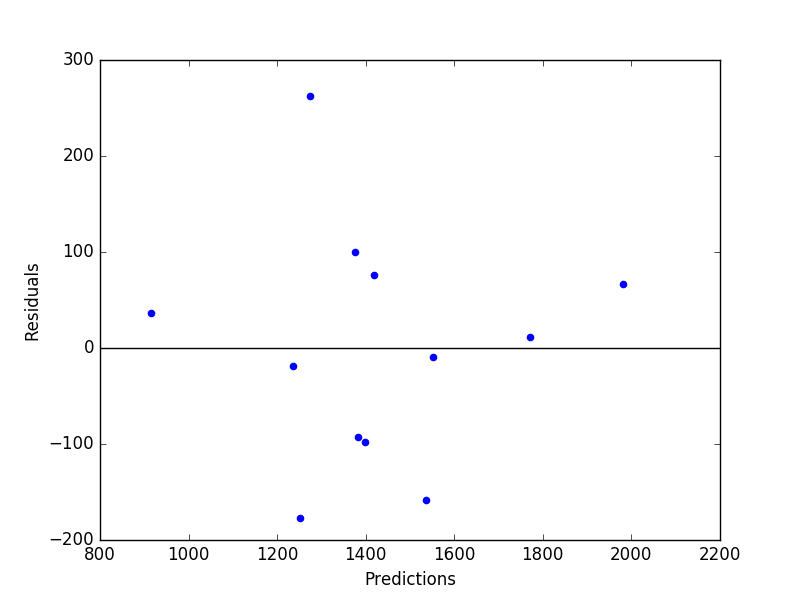
\includegraphics[scale=0.5]{Images/residuals}
\caption{Visual analysis of regression residuals}
\label{fig1}
\end{figure}
The residuals are scattered evenly and randomly showing that they are consistent with random error. This proves that the regression model is systematically correct. In order to clearly illustrate the how well or poorly the system performed, a plot of the expected responses and observed responses was drawn and is shown in Figure 6.2.
\begin{figure}[ht!]
\centering
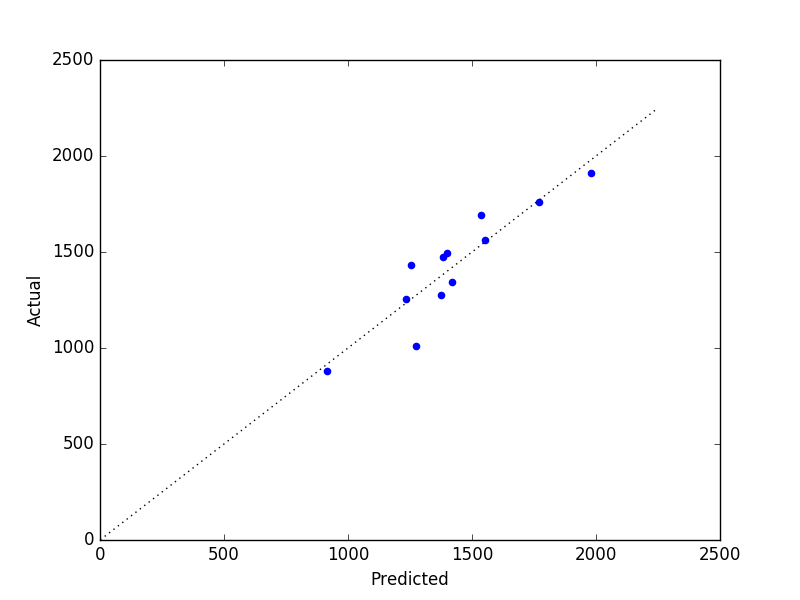
\includegraphics[scale=0.5]{Images/ac_v_pred}
\caption{Plot of expected responses against predicted responses}
\label{fig1}
\end{figure}
While the previous experiments focused more specifically on assessing the quality of the model, this experiment focused more on the big picture of the system, ie. what it predicted compared to what it should have predicted. While the first two experiments asked more of a ``will it work?'' question, this asked more of a ``does it work?'' question. Figure 6.1 shows that nearly half the points were on or just off the line while majority of the remaining points fell fairly close to the line. This proves that the derived grain density function $F$ was reasonably correct.\\ \\
%
However, the derived model could be better were it not for two main factors hindering its performance. The first factor is the fact that only $12$ images were used in training and building the model. By normal standards, this is a very small dataset for a typical supervised learning problem. The second factor is the fact that the expected (or target) responses could not have been very accurate as the number of grain in each image had to manually be counted by eye. Only grains in the foreground and larger than a certain scale were counted. To mitigate the issues arising from this, care was taken to count grains in all the training images in this same manner. All in all, the proposed counting-by-regression system seems to perform well but it is hard to say for sure without more images.
%experiments and results and discuss

\section{Evaluating the Counting-by-Detection Approach}
\subsection{The Model Setup}
The model used for the prediction (and in essence, detection) of grains was the artificial neural network using the Multi-Layer Perceptron (MLP) learning algorithm. The MLP made use of the \textit{\textbf{sigmoid function $\sigma$}} (also known as the \textbf{\textit{logistic function}}) as its activation function \cite{REF28}. The sigmoid function is as follows:
\begin{equation}
\sigma(x) = \frac{1}{1 + e^{-x}}
\end{equation}
The MLP used \textit{\textbf{backpropagation by means of the stochastic gradient descent}} algorithm for tuning its weights \cite{REF29}. Neural networks possess a number of \textit{hyperparameters} which cannot be learned by fitting the model to the data but could influence their performance greatly. In particular, the MLP neural network used for this task had the following hyperparameters:
\begin{itemize}
\item \textit{hidden layer arrangement} - This refers to the number of hidden layers in the network as well as the number of neurons in each layer.
\item \textit{alpha} - This is the \textit{L2} regularization penalty for minimizing prediction error
\item \textit{learning rate} - This controls how quickly the gradient descent algorithm travels down the slope to find the minimum of the cost function when tuning the weights of the neurons.
\item \textit{batch size} - This refers to the size of the mini-batches chosen by the stochastic gradient descent algorithm to speed up the learning process.
\end{itemize}
In order to get the best performance from the MLP, an attempt was made to determine the optimum values for these hyperparameters. To do this, the \textit{\textbf{Grid Search}} algorithm for hyperparameter optimization was employed. Grid search is simply an exhaustive search through a manually specified subset of the hyperparameter space \cite{REF30}.

\subsection{Evaluation Methodology}
350 images were hand selected and labeled to form a data set. The images were selected in a balanced manner with roughly the same amount of instances of all classes. All of this data was used for training and building the neural network. The same data was also used in evaluating the performance of the neural network. Things were done this way because while there was no shortage of sub-images, they had to be labeled manually. Labeling more sub-images for testing than the 350 images already labeled would have been a time-consuming process. On the other hand, we thought it would have been unwise to split the data into separate training and testing sets as the dataset was not very large to begin with. To overcome this problem, \textit{cross validation} was used for evaluation. Cross validation aims to define a dataset to ``test'' a model in the training phase, in order to limit problems like overfitting and give an idea of how the model will generalize to an independent dataset. In addition to this, the \textit{sensitivity} and \textit{specificity} of the classifier used for grain detection was also calculated and used as an evaluation metric. Sensitivity and specificity are statistical metrics used to evaluate binary classification problems. Sensitivity (also known as recall or true positive rate) measures the proportion of positive instances that are correctly identified as such. Similarly, specificity (also known as true negative rate) measures the proportion of negative instances that are correctly identified as such. Mathematically, they can be expressed as follows:
\begin{equation}
sensitivity = \frac{\text{number of true positives}}{\text{number of true positives + number of false negatives}} 
\end{equation}
\begin{equation}
specificity = \frac{\text{number of true negatives}}{\text{number of true negatives + number of false positives}} 
\end{equation}
Sensitivity estimates how well a classifier avoids false negatives while specificity estimates how well it avoids false positives. A perfect classifier would have $100\%$ sensitivity and $100\%$ specificity, that is, a high sensitivity and an equally high specificity. However, in practice there is usually a trade-off between the two.



\bigskip

%%% ----------------------------------------------------------------------
\goodbreak

\subsection{System Performance}
For evaluating the accuracy of our MLP classifier, 5-fold cross validation was used. The data was split into five sets and five iterations of the following procedure were carried out. At each iteration, one set was selected to be the training set (used to build the classifier) and the remaining four were used to test the classifier. The set selected as the training set was changed in each of the five iterations. Once all the iterations were completed, the accuracies from each one was averaged to give the mean accuracy of the classifier. This was needed to get as good a classifier as possible. This is because MLP neural networks start with random weights assigned to the neurons. The values of these starting weights affect the weights that the MLP ends up with, thereby affecting its performance. To get the best model possible, the neural network was built (with random weights) $n$ times. After each build, it was evaluated using the 5-fold cross validation strategy to paint a picture of its accuracy. The MLP with the best accuracy (found to be $80.68\%$) was selected and serialized to disk to be used as the model as needed.\\ \\
%
Once constructed, the characteristics of the model are evaluated by calculating its sensitivity (true positive rate) and specificity (true negative rate). This gives a better idea of how the classifier performs in a more generalized sense. Table 6.1 shows a confusion matrix illustrating the results of applying the classifier to a test set of sub-images independent from the ones used to train and validate it. From this, we were able to calculate the sensitivity and specificity for the final model after crossvalidation and gridsearching the space of the hyperparameters to produce the optimum model. The final classifier had a sensitivity of $72\%$ and a specificity of $90\%$. From the confusion matrix and sensitivity and specificity metrics, it can be seen that while the classifier performs fairly well in identifying sub-images that contain grains, it is better at identifying sub-images that do not contain grains.     
\begin{table}[ht!]
\begin{center}
    \begin{tabular}{l|l|c|c|c}
    \multicolumn{2}{c}{}&\multicolumn{2}{c}{Expected Response}&\\
    \cline{3-4}
    \multicolumn{2}{c|}{}&True&False&\multicolumn{1}{c}{Total}\\
    \cline{2-4}
    \multirow{2}{*}{Observed Response}& True & \cellcolor{green!25}TP $(34)$ & FP $(4)$ & $38$\\
    \cline{2-4}
    & False & FN $(13)$ & \cellcolor{green!25}TN $(37)$ & $50$\\
    \cline{2-4}
    \multicolumn{1}{c}{} & \multicolumn{1}{c}{Total} & \multicolumn{1}{c}{$47$} & \multicolumn{1}{c}{$41$} & \multicolumn{1}{c}{$N = 88$}\\
    \end{tabular}
\end{center}
\caption{Confusion matrix for grain classification}
\end{table}
To further examine the general performance of the classifier, a \textit{\textbf{Receiver Operating Characteristic (ROC) curve}} was plotted. An ROC curve is a graphical plot that illustrates the performance of a binary classifier system as its discrimination threshold is varied. Its discrimination threshold refers to the threshold with which it separates predictions into positive and negative responses. The curve was obtained by plotting the true positive rate and the false positive rate ($1 - \text{specificity}$) at varying values of the discrimination threshold. The true positive rate represents how many sub-images are correctly classified as containing a grain while the false positive rate represents how many sub-images are wrongly classified as containing grains. Figure 6.3 shows the ROC curve obtained from varying the discrimination threshold. The ROC curve illustrates the trade-off between true positives and false positives. A perfect classifier would yield a point in the upper left corner or coordinate (0,1) of the ROC space, representing 100\% sensitivity (no false negatives) and 100\% specificity (no false positives). This means the closer to the top the curve lies, the better the classifier. Our classifier lies fairly close to the top left, further illustrating that it performs reasonably well.
\begin{figure}[ht!]
\centering
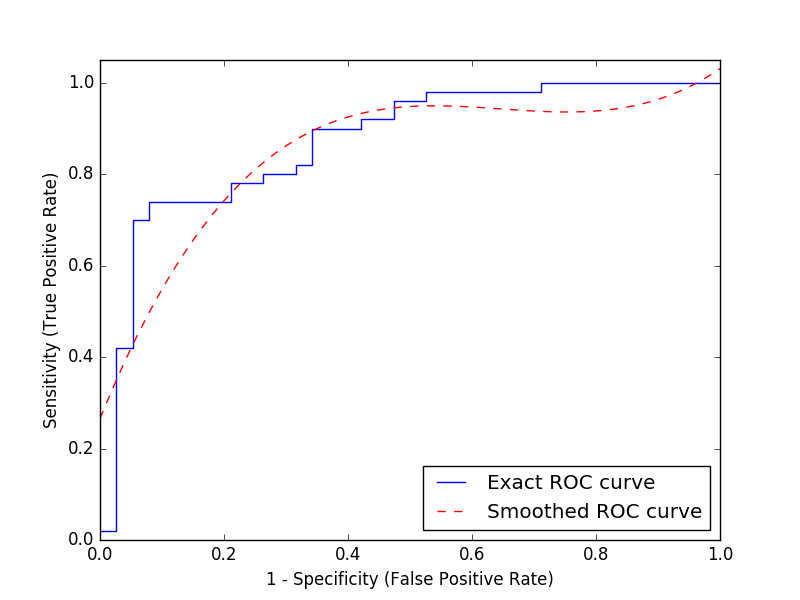
\includegraphics[scale=0.5]{Images/roc.png}
\caption{Receiver Operating Characteristic (ROC) curve}
\label{fig1}
\end{figure}
%
Having determined that the classifier could detect grains in images with an accuracy of $80.68\%$, it would be interesting to find out what this meant for the counting system itself. Tables 6.2 and 6.3 show the actual and predicted counts for the images provided as well as the time taken for the system to compute the counts. From these tables, it can be seen that the system seemed to perform better on certain kinds of images than others. This was due to the fact that in the ROI extraction stage, the clusters to be extracted from the original image were hardcoded. This caused problems because the hardcoded clusters were not always the optimum (or sometimes even particularly good) clusters to select as regions of interest. A way around this problem would be to manually select the clusters denoting regions of interest to be extracted before passing a query image to the system. A simple interactive program was written to this end. Figure 6.4 shows a screenshot of the ROI extraction interface. The program allows a user to upload an image and set the number of clusters that they wish to detect using the k-means clustering algorithm. The program then displays the image with the clusters overlayed over it and the user is able to select the clusters that they would like to extract. While this method might be slightly labour-intensive when a medium to large number of images need to have their grains counted, it yields much better performance. The trade-off here between labour-intensiveness and performance is something that would need to be considered in practice.
\begin{figure}[ht!]
\centering
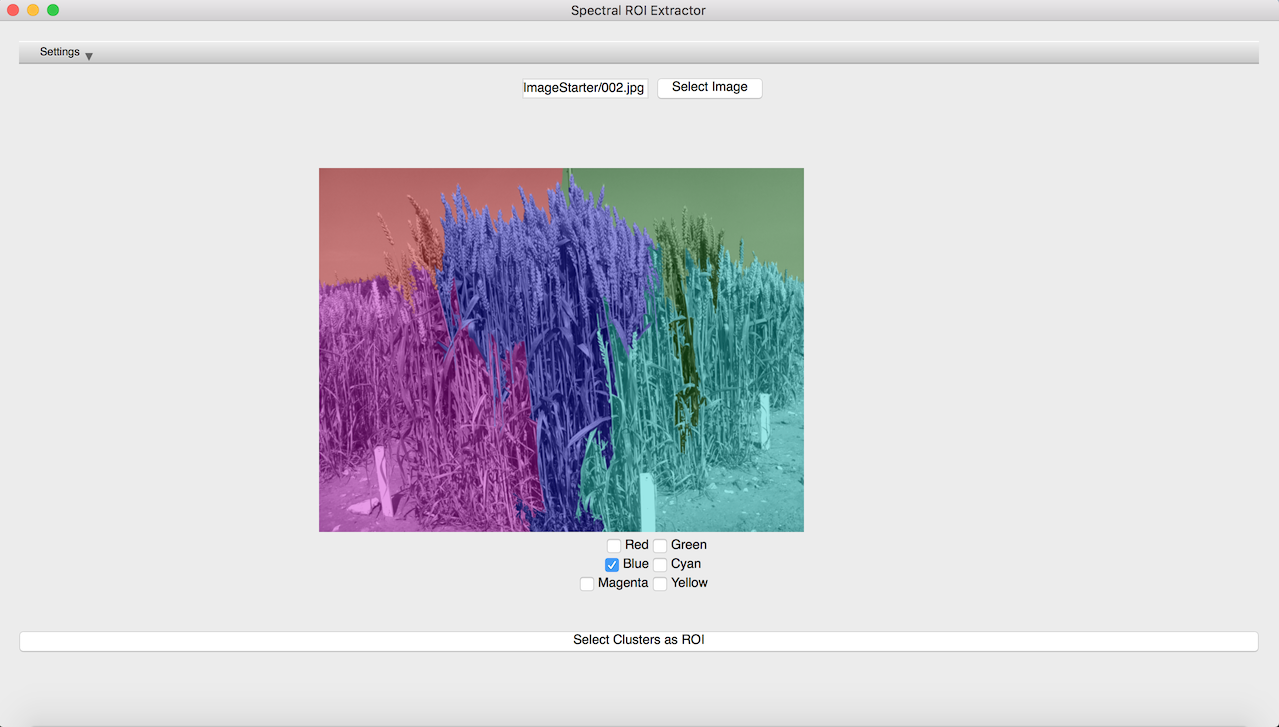
\includegraphics[scale=0.7]{Images/gui}
\caption{Interactive program for manual ROI extraction}
\label{fig1}
\end{figure}

\bigskip

%%% ----------------------------------------------------------------------
\goodbreak

\section{Thoughts and Comparisons}
It was difficult to properly evaluate the counting-by-regression approach. While it showed poorer results by being off the actual count by more than the counting-by-detection method, it should be noted that it only had a dataset consisting of $12$ images. Using only $12$ images would definitely not have built a very good model. The counting-by-detection approach on the other hand had access to 5000 potential examples from each wheat image. Therefore, while the counting-by-detection approach out-performed the counting-by-regression approach, it is still too soon to write off the regression approach as being inferior. However, because we know the accuracy of regression approaches is limited as there is no universal function that can map images to grain counts for any and all images. On the other hand, if a system can correctly detect grains in images (of any kind) to a reasonable extent, such a system would outclass any built on regression approaches.\\ \\
%
The counting-by-detection system proposed relies on a machine learning classifier for grain detection. Our solution makes use of a neural network. We tried other classifiers to see how they all measured up. For image classification, neural networks and support vector machines perform best so the two were pit against each other in order to determine which was best for this problem. In particular, an MLP neural network and an SVM with the \textit{radial basis function} as the kernel function were used. While the SVM was hundreds of times faster than the neural network, it only yielded a prediction accuracy of $65.9\%$ while the neural network yielded an accuracy of $80.68\%$. Despite the fact that the SVM was able to count grains in a fraction of the time that the neural network did, the difference in prediction accuracy was too great to be disregarded in favour of speed. There are still more kinds of neural networks besides the MLP variation used in our solution and in the future, we intend to look into how they can be applied to the problem. Convolutional neural networks are one such example.\\ \\
%
Also, for the proposed counting-by-detection approach, the size of the kernel used for its sub-image extraction is an important component that will be needed to be considered in practice. In our implementation, we have used a kernel of size $20$-by-$20$. This size suits the data used in this project. For the scale of our images, this is an adequate size. Also, all of our images were taken from the same distance so had the same scale. This means that the same kernel size could be used for all the images. However, in practice, the scale of a query image and its contents could vary from that of the images observed in training. This means that consideration needs to be put into whether or not the kernel size needs to be changed between applications and by how much they need to be changed. There is a simple and naive way of determining how to change the kernel size but it depends on the assumption that the training images are all (around) the same scale. To naively determine the kernel size for a query observation, it is possible to compute the ratio of the scale of the observed image to the training image. The ratio can then be multiplied by the width and height of the kernel in order to scale it up or down.

\begin{table}[hp!]
  \centering
  \begin{tabular}{ | c | c | c | c |}
    \hline
    Image & Actual count & Predicted count & Time taken \\ \hline
    \begin{minipage}{.3\textwidth}
      \begin{center}
		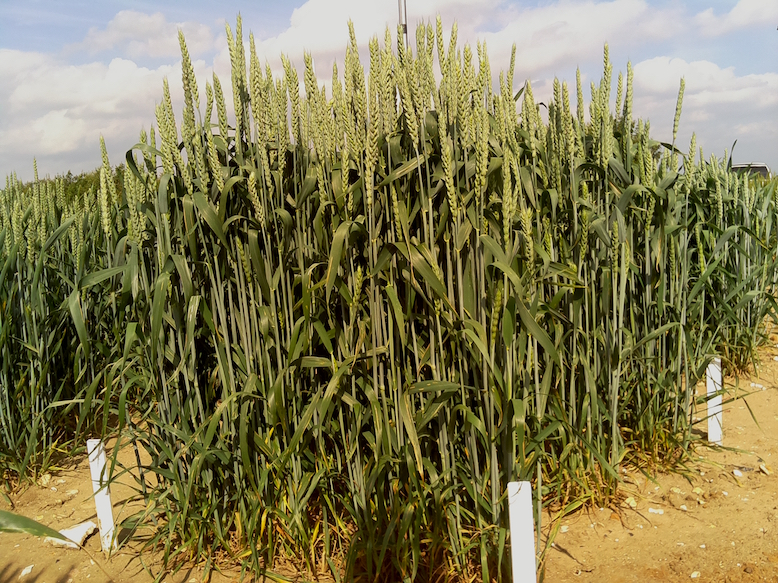
\includegraphics[width=\linewidth]{Images/001}
      \end{center}
    \end{minipage}
    &
    %\begin{minipage}[t]{5cm}
      xxx
    %\end{minipage}
    & 
    %\begin{minipage}{5cm}
      1435
    %\end{minipage}
    & 
    %\begin{minipage}{5cm}
      215
    %\end{minipage}
    \\ \hline
    %%% NEW LINE %%%
    \begin{minipage}{.3\textwidth}
      \begin{center}
		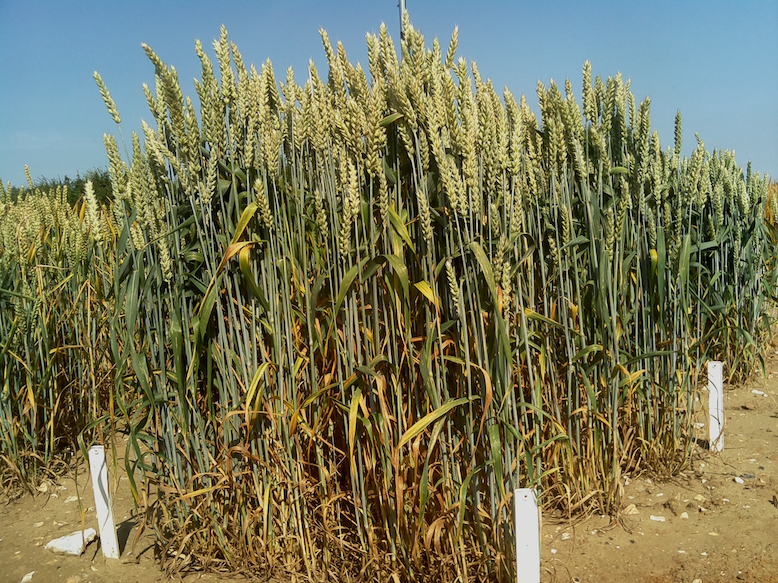
\includegraphics[width=\linewidth]{Images/002}
      \end{center}
    \end{minipage}
    &
    %\begin{minipage}[t]{5cm}
      xxx
    %\end{minipage}
    & 
    %\begin{minipage}{5cm}
      yyy
    %\end{minipage}
    & 
    %\begin{minipage}{5cm}
      zzz
    %\end{minipage}
    \\ \hline
    %%% NEW LINE %%%
    \begin{minipage}{.3\textwidth}
      \begin{center}
		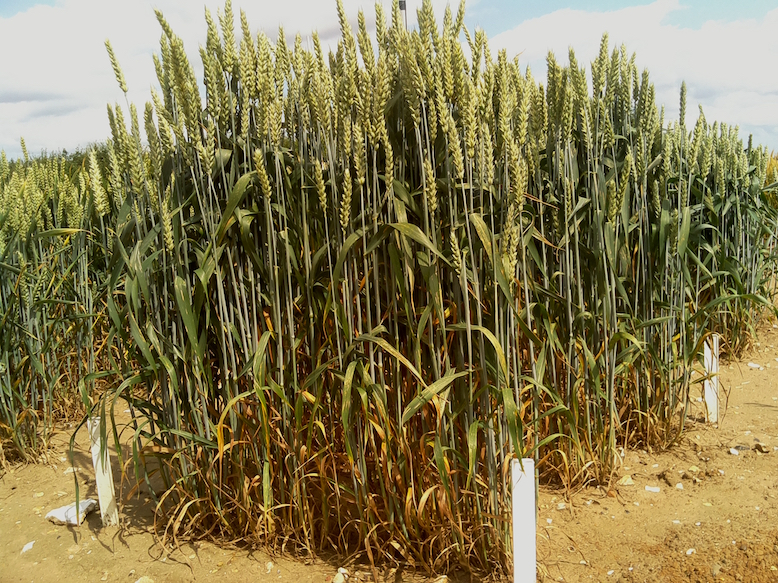
\includegraphics[width=\linewidth]{Images/003}
      \end{center}
    \end{minipage}
    &
    %\begin{minipage}[t]{5cm}
      xxx
    %\end{minipage}
    & 
    %\begin{minipage}{5cm}
      yyy
    %\end{minipage}
    & 
    %\begin{minipage}{5cm}
      zzz
    %\end{minipage}
    \\ \hline
    %%% NEW LINE %%%
    \begin{minipage}{.3\textwidth}
      \begin{center}
		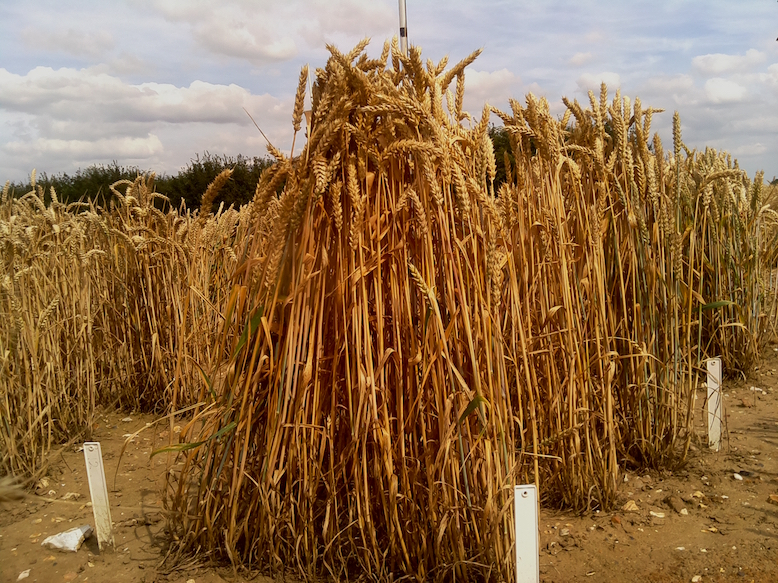
\includegraphics[width=\linewidth]{Images/004}
      \end{center}
    \end{minipage}
    &
    %\begin{minipage}[t]{5cm}
      xxx
    %\end{minipage}
    & 
    %\begin{minipage}{5cm}
      yyy
    %\end{minipage}
    & 
    %\begin{minipage}{5cm}
      zzz
    %\end{minipage}
    \\ \hline
    %%% NEW LINE %%%
    \begin{minipage}{.3\textwidth}
      \begin{center}
		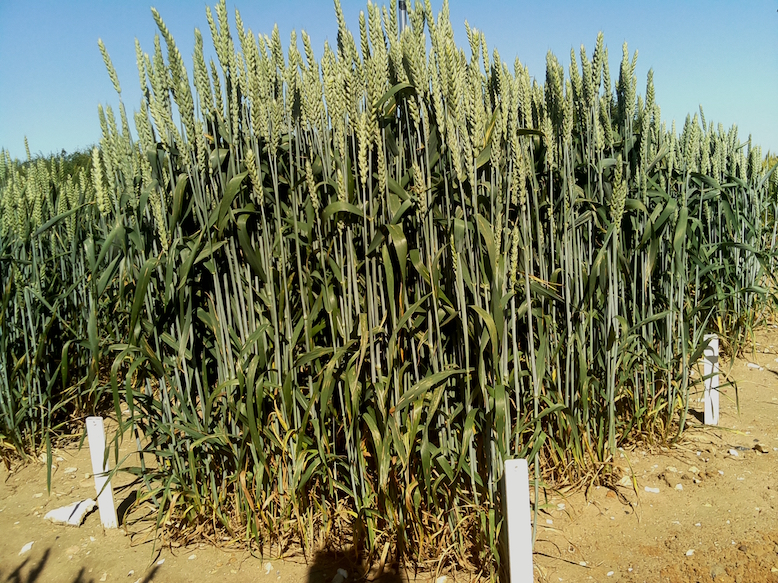
\includegraphics[width=\linewidth]{Images/005}
      \end{center}
    \end{minipage}
    &
    %\begin{minipage}[t]{5cm}
      xxx
    %\end{minipage}
    & 
    %\begin{minipage}{5cm}
      yyy
    %\end{minipage}
    & 
    %\begin{minipage}{5cm}
      zzz
    %\end{minipage}
    \\ \hline
    %%% NEW LINE %%%
    \begin{minipage}{.3\textwidth}
      \begin{center}
		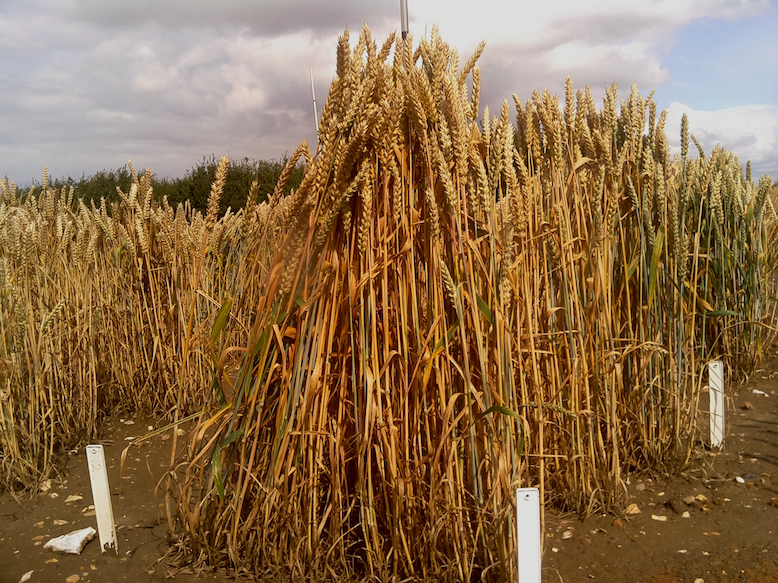
\includegraphics[width=\linewidth]{Images/006}
      \end{center}
    \end{minipage}
    &
    %\begin{minipage}[t]{5cm}
      xxx
    %\end{minipage}
    & 
    %\begin{minipage}{5cm}
      yyy
    %\end{minipage}
    & 
    %\begin{minipage}{5cm}
      zzz
    %\end{minipage}
    \\ \hline
  \end{tabular}
  \caption{Results of proposed system}\label{tbl:myLboro}
\end{table}

%%%%%%%%%%%%%%%%%%%%%%%%%%%%%%%%%%%%%%%%%%%%%%%%%%%%%%%%%%%%%
%%%% table pt 2 
%%%%%%%%%%%%%%%%%%%%%%%%%%%%%%%%%%%%%%%%%%%%%%%%%%%%%%%%%%%%%

\begin{table}[ht!]
  \centering
  \begin{tabular}{ | c | c | c | c |}
    \hline
    Image & Actual count & Predicted count & Time taken \\ \hline
    \begin{minipage}{.3\textwidth}
      \begin{center}
		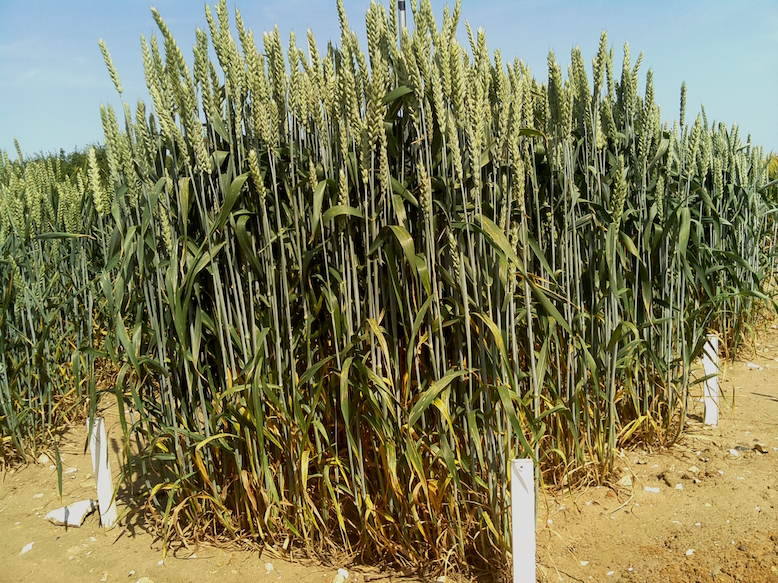
\includegraphics[width=\linewidth]{Images/008}
      \end{center}
    \end{minipage}
    &
    %\begin{minipage}[t]{5cm}
      xxx
    %\end{minipage}
    & 
    %\begin{minipage}{5cm}
      yyy
    %\end{minipage}
    & 
    %\begin{minipage}{5cm}
      zzz
    %\end{minipage}
    \\ \hline
    %%% NEW LINE %%%
    \begin{minipage}{.3\textwidth}
      \begin{center}
		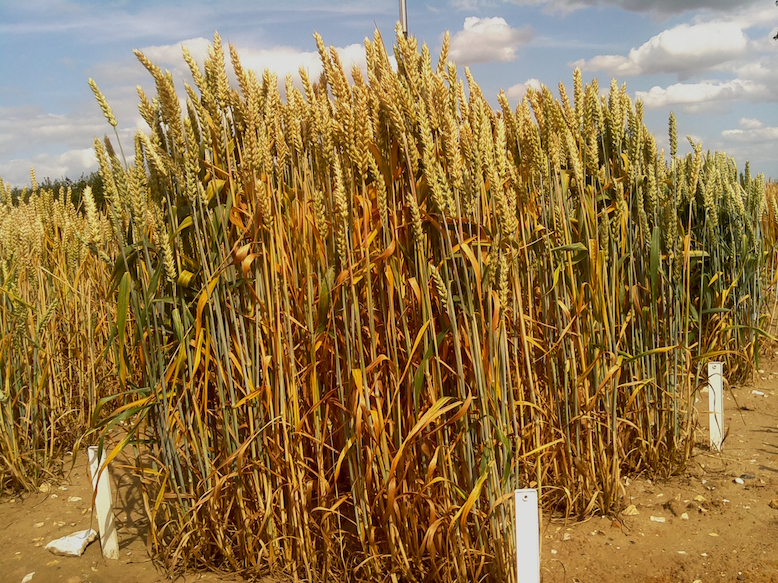
\includegraphics[width=\linewidth]{Images/009}
      \end{center}
    \end{minipage}
    &
    %\begin{minipage}[t]{5cm}
      xxx
    %\end{minipage}
    & 
    %\begin{minipage}{5cm}
      yyy
    %\end{minipage}
    & 
    %\begin{minipage}{5cm}
      zzz
    %\end{minipage}
    \\ \hline
    %%% NEW LINE %%%
    \begin{minipage}{.3\textwidth}
      \begin{center}
		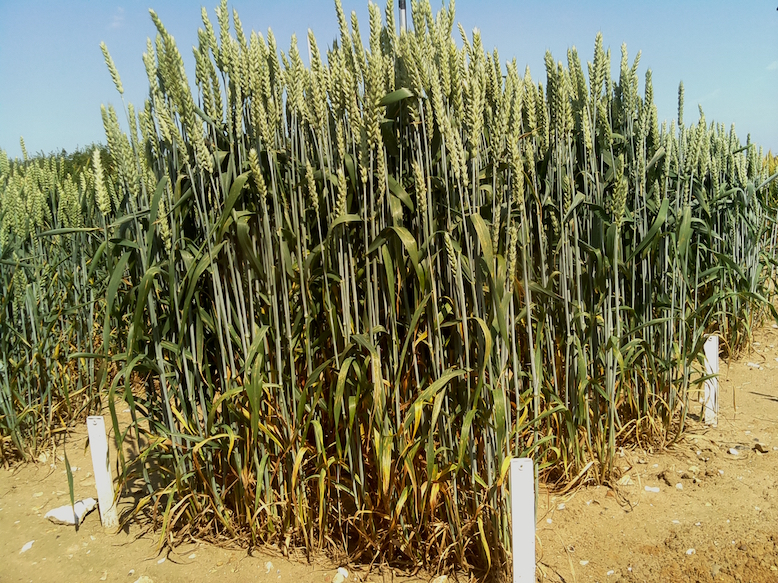
\includegraphics[width=\linewidth]{Images/010}
      \end{center}
    \end{minipage}
    &
    %\begin{minipage}[t]{5cm}
      xxx
    %\end{minipage}
    & 
    %\begin{minipage}{5cm}
      yyy
    %\end{minipage}
    & 
    %\begin{minipage}{5cm}
      zzz
    %\end{minipage}
    \\ \hline
    %%% NEW LINE %%%
    \begin{minipage}{.3\textwidth}
      \begin{center}
		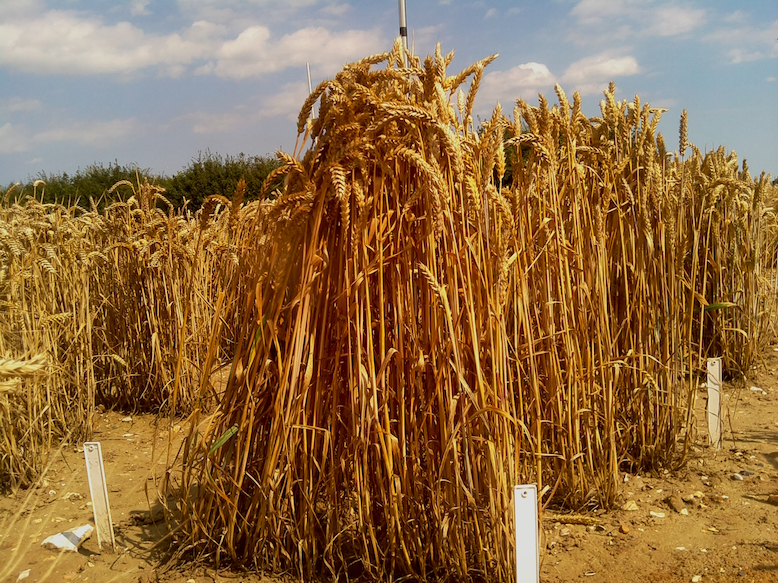
\includegraphics[width=\linewidth]{Images/011}
      \end{center}
    \end{minipage}
    &
    %\begin{minipage}[t]{5cm}
      xxx
    %\end{minipage}
    & 
    %\begin{minipage}{5cm}
      yyy
    %\end{minipage}
    & 
    %\begin{minipage}{5cm}
      zzz
    %\end{minipage}
    \\ \hline
    %%% NEW LINE %%%
    \begin{minipage}{.3\textwidth}
      \begin{center}
		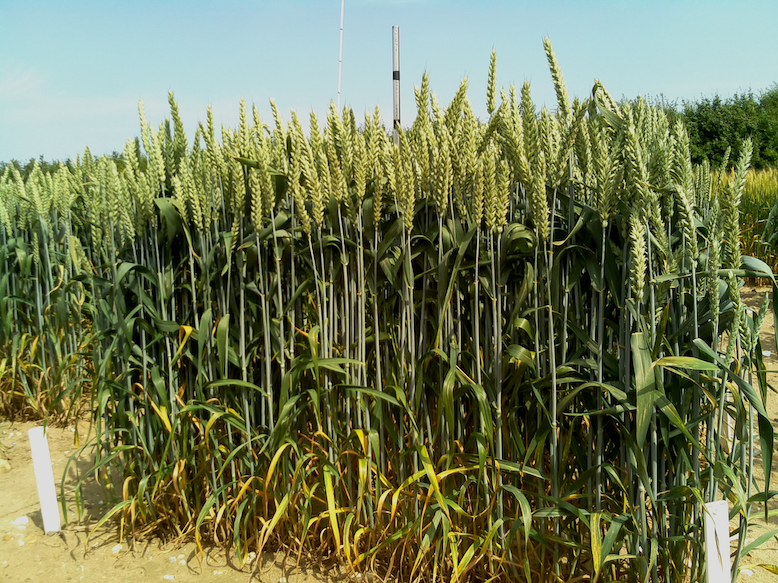
\includegraphics[width=\linewidth]{Images/012}
      \end{center}
    \end{minipage}
    &
    %\begin{minipage}[t]{5cm}
      xxx
    %\end{minipage}
    & 
    %\begin{minipage}{5cm}
      yyy
    %\end{minipage}
    & 
    %\begin{minipage}{5cm}
      zzz
    %\end{minipage}
    \\ \hline
    %%% NEW LINE %%%
  \end{tabular}
  \caption{Results of proposed system}\label{tbl:myLboro}
\end{table}

\bigskip

%%% ----------------------------------------------------------------------



